%%%%%%%%%%%%%%%%%%%%%%%%%%%%%%%%%%%%%%%%%
% Short Sectioned Assignment
% LaTeX Template
% Version 1.0 (5/5/12)
%
% This template has been downloaded from:
% http://www.LaTeXTemplates.com
%
% Original author:
% Frits Wenneker (http://www.howtotex.com)
%
% License:
% CC BY-NC-SA 3.0 (http://creativecommons.org/licenses/by-nc-sa/3.0/)
%
%%%%%%%%%%%%%%%%%%%%%%%%%%%%%%%%%%%%%%%%%

%----------------------------------------------------------------------------------------
%	PACKAGES AND OTHER DOCUMENT CONFIGURATIONS
%----------------------------------------------------------------------------------------

\documentclass[paper=letter, fontsize=11pt]{scrartcl} % A4 paper and 11pt font size

\usepackage[T1]{fontenc} % Use 8-bit encoding that has 256 glyphs
%\usepackage{fourier} % Use the Adobe Utopia font for the document - comment this line to return to the LaTeX default
\usepackage[english]{babel} % English language/hyphenation
\usepackage{amsmath,amsfonts,amsthm} % Math packages

\usepackage{enumitem}

\usepackage{sectsty} % Allows customizing section commands

%these two packages are needed for xfig 
\usepackage[dvips,final]{graphicx}
\usepackage{color} %include even if images aren’t in color

\usepackage{float}
%\floatstyle{boxed} 
\usepackage[export]{adjustbox}
\restylefloat{figure}

\usepackage{listings}
\lstset{
  basicstyle=\footnotesize\ttfamily,breaklines=true,      % the size of the fonts that are used for the code
  commentstyle=\color{mygreen},    % comment style
}

\allsectionsfont{\centering \normalfont\scshape} % Make all sections centered, the default font and small caps

\usepackage{fancyhdr} % Custom headers and footers
\pagestyle{fancyplain} % Makes all pages in the document conform to the custom headers and footers
\fancyhead{} % No page header - if you want one, create it in the same way as the footers below
\fancyfoot[L]{} % Empty left footer
\fancyfoot[C]{\thepage} % Empty center footer
\fancyfoot[R]{} % Page numbering for right footer
\renewcommand{\headrulewidth}{0pt} % Remove header underlines
\renewcommand{\footrulewidth}{0pt} % Remove footer underlines
\setlength{\headheight}{13.6pt} % Customize the height of the header

%\numberwithin{equation}{section} % Number equations within sections (i.e. 1.1, 1.2, 2.1, 2.2 instead of 1, 2, 3, 4)
%\numberwithin{figure}{section} % Number figures within sections (i.e. 1.1, 1.2, 2.1, 2.2 instead of 1, 2, 3, 4)
%\numberwithin{table}{section} % Number tables within sections (i.e. 1.1, 1.2, 2.1, 2.2 instead of 1, 2, 3, 4)

\setlength\parindent{0pt} % Removes all indentation from paragraphs - comment this line for an assignment with lots of text

%----------------------------------------------------------------------------------------
%	TITLE SECTION
%----------------------------------------------------------------------------------------

\newcommand{\horrule}[1]{\rule{\linewidth}{#1}} % Create horizontal rule command with 1 argument of height

\title{	
\normalfont \normalsize 
\textsc{University of Lethbridge} \\ [25pt] % Your university, school and/or department name(s)
\horrule{0.5pt} \\[0.4cm] % Thin top horizontal rule
\huge Computational Optimization Term Project Report\\ % The assignment title
\horrule{2pt} \\[0.5cm] % Thick bottom horizontal rule
}

\author{Ahamad Imtiaz Khan\\ID:001188188} % Your name

\date{\normalsize\today} % Today's date or a custom date

\begin{document}

\maketitle % Print the title



\Large \textbf{1. Problem Statement:}
\normalsize Sarah is an Operation Management Student of Takshashila University (TU). In her 
last semester she will need to take some courses. Some courses are compulsory and some courses have choices.
For choosing the courses Sarah needs to fulfil some conditions. They are stated  bellow:
    
\begin{enumerate} [align=left,style=nextline,leftmargin=1.5cm,labelsep=\parindent,font=\normalfont]
\item[i.] She needs to take 5 courses in total.
\item[ii.] She needs to take Business Strategy (MGT 490) and International Finance (FIN 358).
\item[iii.] She has interest in service-learning course and found Intergenerational Computing (CIS 102T) and Web Design for Non-profit Organizations (CIS 102W) interesting. She needs to take one of the two courses 
between these.
\item[iv.] Among four potential finance elective courses [Data Analysis in Finance (FIN 325);
 Risk Management(FIN 352); Options, Futures, and Swaps (FIN 356) and 
Fixed Instruments and Markets (FIN 359)] she needs to take two courses.
\end{enumerate}

Sarah rated each section of the available courses based on content of the course, reputation of the instructor and timing of the course. Now it's my job to find an appropriate schedule for Sarah that will meet all the above mentioned conditions and also will give highest total rating. I will solve the problem using two strategies. First one is Greedy Heuristic and the second one is LP model. Using Greedy Heuristic I will find a solution which may not be optimal but good enough, using LP model I will find optimal solution and finally I will find maximum rating of three days a week schedule by extending the LP .
\newline
\newline
\Large \textbf{2. Input Data:}
\normalsize The input data for the problem are rearranged as follows: 

\begin{table}[h]
\begin{center}
    \resizebox{\textwidth}{!}{\begin{tabular}{| l | l | l | l | l | l | l | l | l |}
  
    \hline
    Meeting Time(s) & MGT 490 & FIN 358 & CIS 102T & CIS 102W & FIN 325 & FIN 352 & FIN 356 & FIN 359 \\ \hline
    M 6-8:45 p.m. & 4.3 & 0 & 0 & 0 & 0 & 3.6 & 0 & 3 \\ \hline
    T 6-8:45 p.m. & 3.8 & 0 & 0 & 3.7 & 0 & 0 & 3.2 & 0 \\ \hline
    W 6-8:45 p.m. & 3.5 & 3.5 & 0 & 0 & 0 & 0 & 0 & 3.5 \\ \hline
    F 6-8:45 p.m. & 3.5 & 0 & 0 & 0 & 0 & 0 & 0 & 0 \\ \hline
    \shortstack[l]{M 1:25-2:20 p.m. \\ W 1:25-3:15 p.m.} & 4.6 & 0 & 0 & 0 & 3.7 & 0 & 0 & 0 \\ \hline
    \shortstack[l]{T 1:25-3:15 p.m. \\ Th 1:25-2:20 p.m.} & 2.7 & 3.3 & 0 & 0 & 0 & 0 & 3.4 & 0 \\ \hline
    W 2:30-5:15 p.m. & 0 & 0 & 4.4 & 3.5 & 0 & 0 & 0 & 0 \\ \hline
    Th 2:30-5:15 p.m. & 0 & 0 & 3.1 & 0 & 0 & 0 & 0 & 0 \\ \hline
    Th 6-8:45 p.m. & 0 & 0 & 0 & 0 & 3 & 0 & 0 & 0 \\ \hline
    \shortstack[l]{M 1:25-3:15 p.m. \\ W 1:25-2:20 p.m.} & 0 & 0 & 0 & 0 & 0 & 3.9 & 0 & 0 \\ \hline
    
    \end{tabular}}
    \end{center}

\caption{Course Data}

\end{table}

Table 1 shows the rating of the sections of corresponding subjects and their meeting times. Ratings of sections of a subject are in the same column under the subject code and the corresponding rows indicates the meeting times of the sections. For example MGT 490 has 6 sections and the first section has rating of 4.3 and its meeting time is M 6-8:45 p.m.
\newline
\newline
\Large \textbf{3. Solution Strategies:}\\
\newline
 \normalsize \textbf{a. Heuristic:}
Solving the scheduling problem using Greedy Heuristic is simple and straight forward. The concept of greedy heuristic is I have to choose local maximum rating at each iteration. Finally I will get total rating. The things I need to keep in my mind are:  
\begin{enumerate}[align=left,style=nextline,leftmargin=1.5cm,labelsep=\parindent,font=\normalfont]
\item[i.] The program should meet the conditions stated in Problem Statement.
\item[ii.] There are some meeting times that conflict with each other. So if I choose a maximum rating in any iteration and it's meeting time(s) conflicts with any other meeting time(s) then I will not consider the ratings under that/those meeting time(s) in the next iterations.
\end{enumerate}  

I put the course codes, meeting times and the ratings in a text file and from octave function I read the data and stored course codes, meeting times and ratings in three matrices. From the matrix in which I stored ratings I calculated maximum rating of each column in every iteration. Maximum rating of a column indicates the maximum rating of that subject. After getting the maximum rating I made all indices of that row to zero because the corresponding time slot is taken, so other ratings in the same row will not contribute in finding maximum ratings in the following iterations. If the time slot conflicts with any other time slot(s) the ratings of the corresponding row(s) also made zero for same reason. Finally I got the maximum ratings of each subjects and choose the ratings of five subjects that met Sarah's conditions and showed the output in readable format. The maximum rating using greedy heuristic is 18.8.
The output from octave console is given bellow:

\begin{figure}[H]
  
  \centering
  \frame{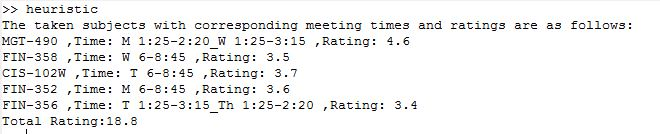
\includegraphics[width=0.8\textwidth]{heuristic}}
    
    \caption{Output of Greedy Heuristic}
\end{figure}

The Octave code for greedy heuristic is attached in appendix part.
\newline
\newline
 \normalsize \textbf{b. LP:} 
Now I will use LP model to find an optimal solution. In my case it is a schedule that will produce maximum rating. In other word I can say that I have to maximize.
\begin{center}
 $\displaystyle\sum_{i=1}^{10}\sum_{j=1}^{8} c_{ij}x_{ij}$
\end{center}

Here c is matrix of coefficients  and x is matrix of decision variables. In this case Table 1 represents c and Table 2 represents x  

\begin{table}[h]
\begin{center}
    \resizebox{0.95\textwidth}{!}{\begin{tabular}{| l | l | l | l | l | l | l | l | l |}
  
    \hline
    Meeting Time(s) & MGT 490 & FIN 358 & CIS 102T & CIS 102W & FIN 325 & FIN 352 & FIN 356 & FIN 359 \\ \hline
    M 6-8:45 p.m. & 1/0 & 1/0 & 1/0 & 1/0 & 1/0 & 1/0 & 1/0 & 1/0 \\ \hline
    T 6-8:45 p.m. & 1/0 & 1/0 & 1/0 & 1/0 & 1/0 & 1/0 & 1/0 & 1/0 \\ \hline
    W 6-8:45 p.m. & 1/0 & 1/0 & 1/0 & 1/0 & 1/0 & 1/0 & 1/0 & 1/0 \\ \hline
    F 6-8:45 p.m. & 1/0 & 1/0 & 1/0 & 1/0 & 1/0 & 1/0 & 1/0 & 1/0 \\ \hline
    \shortstack[l]{M 1:25-2:20 p.m. \\ W 1:25-3:15 p.m.} & 1/0 & 1/0 & 1/0 & 1/0 & 1/0 & 1/0 & 1/0 & 1/0 \\ \hline
    \shortstack[l]{T 1:25-3:15 p.m. \\ Th 1:25-2:20 p.m.} & 1/0 & 1/0 & 1/0 & 1/0 & 1/0 & 1/0 & 1/0 & 1/0 \\ \hline
    W 2:30-5:15 p.m. & 1/0 & 1/0 & 1/0 & 1/0 & 1/0 & 1/0 & 1/0 & 1/0 \\ \hline
    Th 2:30-5:15 p.m. & 1/0 & 1/0 & 1/0 & 1/0 & 1/0 & 1/0 & 1/0 & 1/0 \\ \hline
    Th 6-8:45 p.m. & 1/0 & 1/0 & 1/0 & 1/0 & 1/0 & 1/0 & 1/0 & 1/0 \\ \hline
    \shortstack[l]{M 1:25-3:15 p.m. \\ W 1:25-2:20 p.m.} & 1/0 & 1/0 & 1/0 & 1/0 & 1/0 & 1/0 & 1/0 & 1/0 \\ \hline
    
    \end{tabular}}
    \end{center}

\caption{Decision Variables}
\end{table}

If any course is taken in $(i,j)^{th}$ position then that  $x_{ij}$ is 1 otherwise it's 0. So my task is to maximize 
$\displaystyle\sum_{i=1}^{10}\sum_{j=1}^{8} c_{ij}x_{ij}$ which is actually sum of product of Table 1 and Table 2.

I used excel solver to solve the LP, unlike heuristic I had to introduce some other constraints. All the constraints that must meet to solve the LP are given bellow:

\begin{enumerate}[align=left,style=nextline,leftmargin=1.5cm,labelsep=\parindent,font=\normalfont]
\item[i.]  Each course cannot be taken more than once.
\item[ii.] Not more than one class can be chosen from one meeting time.
\item[iii.] There are some meeting times that conflicts with each other. At most one class can be taken from those conflicting time slots.  
\item[iv.] MGT 490 and FIN 358 must be taken.
\item[iv.] Number of course between CIS 102T and CIS 102W is one.
\item[v.] Number of courses between FIN 325, FIN 352, FIN 356 and FIN 359 is two.
\item[vi.] Total number of course is five.
\end{enumerate}  

All the above mentioned constraints were added using excel solver. Here is an example how I added constraint in excel solver. Let us consider constraint (vi). There are four columns for FIN 325, FIN 352, FIN 356 and FIN 359. I must choose at most two courses from these four. So summation of these four columns is equal to two and as I cannot take one course more than once so summation of each column is less than or equal to zero. I added the other constraints in similar ways in excel solver.  The resulting decision variables with coefficients and optimal objective function are shown in Figure 2. Meeting time constraints, Course constraints are shown in Figure 3. Objective function is sum of products of the elements of Table 1 and 2. After solving this problem in excel solver I get the optimal rating for this LP which is 19.5.         
\begin{figure}[H]
  
  \centering
     \frame{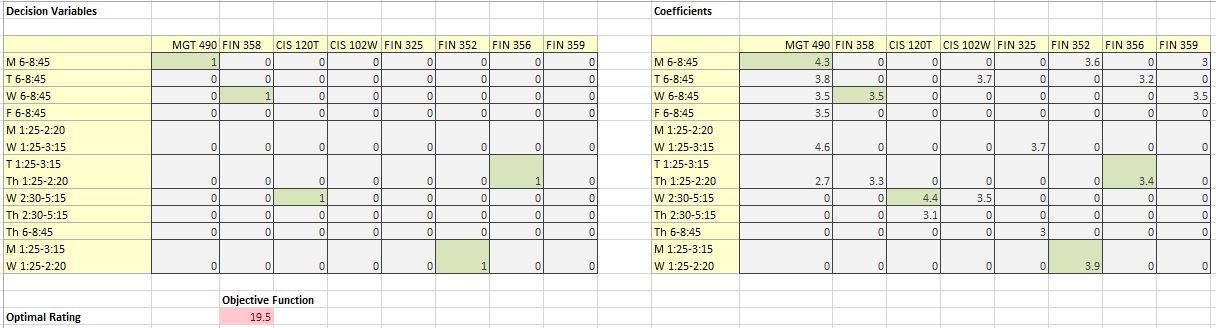
\includegraphics[width=1.0\textwidth, height=0.3\textheight]{decision}}
    \caption{Resulting Decision variables, Coefficients and Optimal Objective function}
\end{figure}

\begin{figure}[H]
  
  \centering
    \frame{ 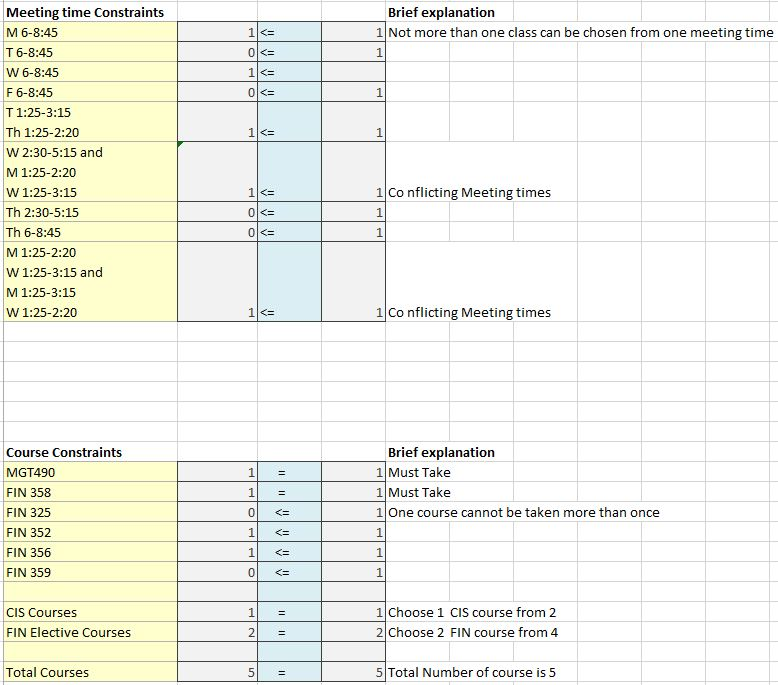
\includegraphics[width=0.8\textwidth, height=0.5\textheight]{constraints}}
    \caption{Meeting time constraints and Course constraints}
\end{figure}

Using excel solver I also found the shadow prices (dual values) of this LP. I copied the shadow prices beside the constraints. They are as follows:

\begin{figure}[H]
  
  \centering
    \frame{ 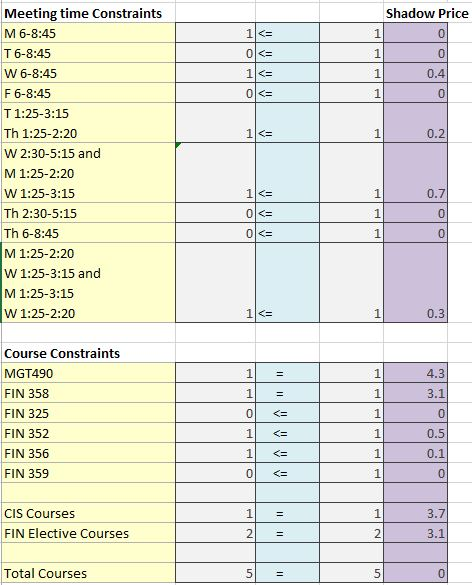
\includegraphics[width=0.6\textwidth, height=0.34\textheight]{shadow}}
    \caption{Shadow prices (Dual values) of the LP}
\end{figure}
We see that for the meeting time constraints there are some positive non zero shadow prices. But I couldn't found anything meaningful out of these shadow prices as the right hand side of these constraints cannot be increased because Sarah cannot take more than one class in a specific meeting time. It is not possible. By looking at the shadow prices of course constraints we can see that constraints for MGT 490, FIN 358, FIN 352 and FIN 359 have positive non zero values. Again anything meaningful cannot be interpreted from these dual values as the right hand side of these constraints cannot be increased because Sarah will not take same course more than once.\\
Now if we look at the dual values of CIS and FIN elective courses we can see that they are 3.7 and 3.1 respectively so if I increase the rhs of CIS by 1 the resulting rating will be increased by 3.7 and if I increase the rhs of FIN the resulting rating will be increased by 3.1 but in that case I will need to increase the total number of courses. But the dual value for total number of course constraint is 0. In my opinion the dual values cannot be interpreted in any meaningful way.\\  

 \normalsize \textbf{c. Extension:}
In extension part I will introduce new constraints to the LP part and observe what will happen to the optimal rating in extension. The constraint is as follows:
\begin{enumerate}[align=left,style=nextline,leftmargin=1.5cm,labelsep=\parindent,font=\normalfont]
\item[i.]  Without lowering the maximum rating (19.5) too much Sarah wants to see whether she can attend classes only three days a week. 
\end{enumerate}

So I will have some new constraints as well as a new problem. The new problem is, I have to find in which days Sarah will take the classes as well as I will calculate the maximum rating as I calculated earlier. Problem formulation and solution of extension are described bellow:\newline
I have a new row of decision variables. Each cell of that row represents each day of a week. If one or more class is taken on a particular day then the cell is 1 otherwise it's 0. So I added this row as a decision variable in excel solver. (One thing I want to mention here that I kept the constraints and decision variables of the previous LP as it was and added the new decision variables and constraints for this extension)
I added two new constraints for this extension:\\
- Number of classes taken in a specific day of a week is less than or equals to 5.\\
- Total number of days in a week is 3.\\

For example I stored number of classes in each day of a week in a column. Each row of that column actually represents the sum of classes of that specific day. If any class is taken in a specific day of a week then the corresponding cell will become 1 otherwise 0 and the corresponding row in constraint table must be less than or equals to (0/1)*5.  Finally total number of days in a week must be equal to 3. 

After adding the new decision variables and constraints my set of previous decision variables is changed and it looks like as follows.
\begin{figure}[H]
  
  \centering
     \frame{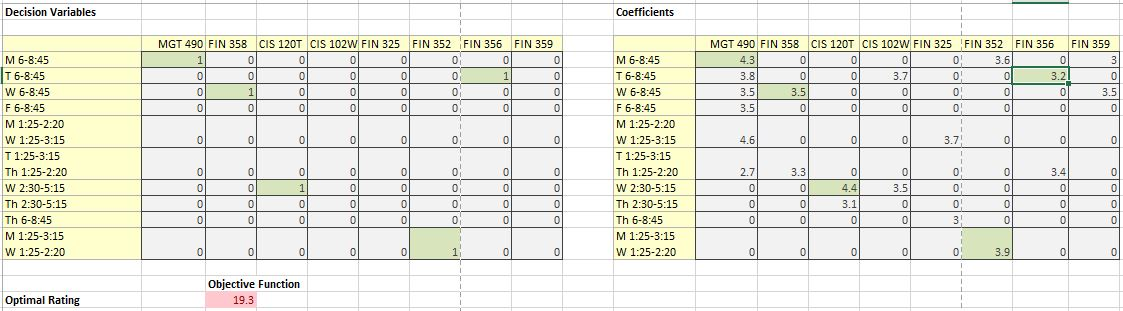
\includegraphics[width=1.0\textwidth]{ext1}}
    \caption{Resulting decision variable, Coefficients and Optimal Objective function for Extension}
\end{figure}
\newline
New decision variables and constraints added for the extension are as follows:

\begin{figure}[H]
  
  \centering
     \frame{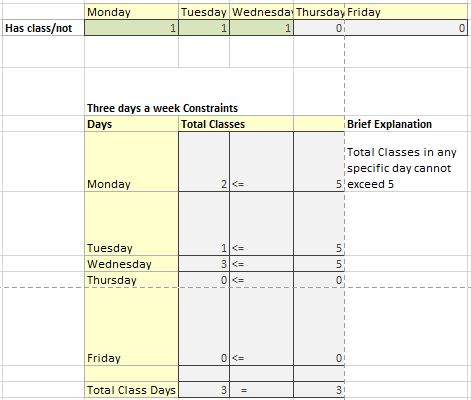
\includegraphics[width=0.6\textwidth, height=0.4\textheight]{ext2}}
    \caption{New decision variables and Constraints for Extension}
\end{figure}
Here the row for Has class/not is for new decision variables that I added with the previous one. Each row of constraint part of Figure 6 is new constraint as well as the total no. of class days in week.\\
Finally I got new maximum rating after imposing three days a week restriction, which is 19.3. It is lower than 19.5 but not that much lower.   


\newpage
\Large \textbf{Appendix:}\\
\newline
 \normalsize \textbf{Octave code for greedy heuristic:}

\begin{lstlisting}
function x = heuristic()
%Read data from file
fileID = fopen('input.txt');
_subjects = textscan(fileID,'%s',1,'Delimiter','#');
_times = textscan(fileID,'%s',1,'Delimiter','#');
sizeA = [8 Inf];
M = fscanf(fileID,'%f %f %f %f %f %f %f %f %f %f %f',sizeA);
M = M'; %Matrix for ratings
fclose(fileID);
[m,n] = size(M);
maxVals = [];
sameTime = [5 7 10;7 5 0;10 5 0]; %Conflicting meeting times

for col=1:n
  [val,maxIndex] =  max(M(:,col));% Find maximum rating from each column 
  maxVals = [maxVals;maxIndex val];
  
  %Deal with conflicticg meeting times   
   if maxIndex == sameTime(1,1)
      for k=1:3
        for l=1:n
          M(sameTime(1,k),l) = 0;
        end
      end
   elseif maxIndex == sameTime(2,1)
      for k=1:3
        for l=1:n
          M(sameTime(2,k),l) = 0;
        end
    end
  
   elseif maxIndex == sameTime(3,1)
      for k=1:3
        for l=1:n
          M(sameTime(3,k),l) = 0;
        end
      end
   else
      %Make the row of max rating zero
      for j=2:n
        M(maxIndex,j) = 0;
      end
  end
  end
  %sorting done for finding 2 FIN selective courses with maximum ratings
  for i=5:8
    for j=5:7
      if maxVals(j,2) < maxVals(j+1,2)
        temp1 = maxVals(j,1);
        temp2 = maxVals(j,2);
        tempSub = _subjects{1}{j};
        maxVals(j,1) = maxVals(j+1,1);
        maxVals(j,2) = maxVals(j+1,2);
        maxVals(j+1,1) = temp1;
        maxVals(j+1,2) = temp2;
        _subjects{1}{j} = _subjects{1}{j+1};
        _subjects{1}{j+1} = tempSub;
      end 
    end
  end
  %Output
  totalRating = maxVals(1,2)+maxVals(2,2)+max(maxVals(3,2),maxVals(4,2))+maxVals(5,2)+maxVals(6,2);
  fprintf('The taken subjects with corresponding meeting times and ratings are as follows:\n');
  fprintf('%s ,Time: %s ,Rating: %1.1f\n',_subjects{1}{1},_times{1}{maxVals(1,1)},maxVals(1,2));
  fprintf('%s ,Time: %s ,Rating: %1.1f\n',_subjects{1}{2},_times{1}{maxVals(2,1)},maxVals(2,2));
  if maxVals(3,2) > maxVals(4,2)
    fprintf('%s ,Time: %s ,Rating: %1.1f\n',_subjects{1}{3},_times{1}{maxVals(3,1)},maxVals(3,2));
  else
    fprintf('%s ,Time: %s ,Rating: %1.1f\n',_subjects{1}{4},_times{1}{maxVals(4,1)},maxVals(4,2));
  end
  fprintf('%s ,Time: %s ,Rating: %1.1f\n',_subjects{1}{5},_times{1}{maxVals(5,1)},maxVals(5,2));
  fprintf('%s ,Time: %s ,Rating: %1.1f\n',_subjects{1}{6},_times{1}{maxVals(6,1)},maxVals(6,2));
  fprintf('Total Rating:%1.1f\n',totalRating);
 end
\end{lstlisting}
%----------------------------------------------------------------------------------------

\vspace{5mm}

 \normalsize \textbf{Input File (input.txt):}
 \begin{lstlisting}
 MGT-490#FIN-358#CIS-120T#CIS-102W#FIN-325#FIN-352#FIN-356#FIN-359
 M 6-8:45#T 6-8:45#W 6-8:45#F 6-8:45#M 1:25-2:20_W 1:25-3:15#T 1:25-3:15_Th 1:25-2:20#W 2:30-5:15#Th 2:30-5:15#Th 6-8:45#M 1:25-3:15_W 1:25-2:20
 4.3 0 0 0 0 3.6 0 3
 3.8 0 0 3.7 0 0 3.2 0
 3.5 3.5 0 0 0 0 0 3.5
 3.5 0 0 0 0 0 0 0 
 4.6 0 0 0 3.7 0 0 0 
 2.7 3.3 0 0 0 0 3.4 0
 0 0 4.4 3.5 0 0 0 0 
 0 0 3.1 0 0 0 0 0 
 0 0 0 0 3 0 0 0 
 0 0 0 0 0 3.9 0 0
 \end{lstlisting}

\end{document}